\documentclass[11pt,a4paper]{report}  % Using 'report' class for structured formatting
\usepackage[utf8]{inputenc}
\usepackage{geometry}
\geometry{margin=1in}
\usepackage{graphicx}
\usepackage{setspace}
\usepackage{titlesec}
\usepackage{tikz}
\usetikzlibrary{shapes.geometric, arrows.meta, positioning, calc}


\setcounter{secnumdepth}{3}
\renewcommand{\thesection}{\arabic{section}}

\begin{document}

% ------------------ Title Page ------------------

\begin{titlepage}

    \centering

    
\includegraphics[width=3.4cm,height=2.6cm ]{College Logo Grayscale.jpg}\\[0.5cm] % Add your college logo file

    \vspace{1cm}
    \textbf{\large A Complex Engineering Problem Report on} \\[0.5cm]
    {\Large \textbf{Constrained-Random and Assertion-Based Layered Testbench for Verification of 5-Port NoC Mesh Router with Virtual Channels using SystemVerilog}}\\[1.5cm]
 {\Large A8451 - SystemVerilog for Verification}\\[1.5cm]
 \textbf{Submitted by}\\ [0.25cm]
 Batch No. {XXXXXXXXXX}

\begin{center}

	\begin{table}[h!]
		\centering
        \setstretch{1}
		\begin{tabular}{l l}

			 {Name of the Student 1} & {Roll No - 1}\\ [2mm]
		{Name of the Student 2} &  {Roll No - 2} \\ [2mm]
			 {Name of the Student 3} &  {Roll No - 3} \\ [2mm]

		\end{tabular}
	\end{table}
\end{center}
 \textbf{Course Facilitator}\\ [0.075in]
     {Course Facilitator Name}\\[0.3cm]
     Assistant Professor\\[3cm]

    { \large\textbf{Department of Electronics and Communication Engineering}}\\[0.5cm]
    { \large\textbf{Vardhaman College of Engineering, Hyderabad}}\\[0.5cm]
    {\large \textbf{September 2026}}

\end{titlepage}


\tableofcontents
\newpage

\section{Introduction}

Functional verification consumes the dominant share of effort in modern
system-on-chip projects, because a single escaped bug can force a multi-million
dollar silicon re-spin. As single shared buses give way to packet-switched
fabrics in many-core chips, the interconnect itself has become one of the
hardest blocks to verify: packets from many ports compete concurrently for the
same outputs under flow control, and directed tests alone cannot cover the
resulting state space \cite{Bergeron}\cite{Spear}.

This Complex Engineering Problem addresses the functional verification of a
parameterized 5-port wormhole Network-on-Chip (NoC) router with two virtual
channels per port, XY routing and round-robin arbitration. A coverage-driven,
layered testbench was developed in SystemVerilog following the layered
methodology of the Verification Methodology Manual: object-oriented components
(Generator, Driver, Monitor, Scoreboard, Coverage) connected through a virtual
interface with clocking blocks and mailboxes, constrained-random stimulus,
SystemVerilog Assertions bound with \texttt{bind}, and functional coverage with
closure \cite{Spear}\cite{UVM}. Simulation was carried out with Synopsys VCS on
EDA Playground across five regression runs totalling 1720 packets and 11846
flits with zero scoreboard errors, as shown in figure \ref{fig:scoreboard}.

\begin{figure}[h!]
    \centering
    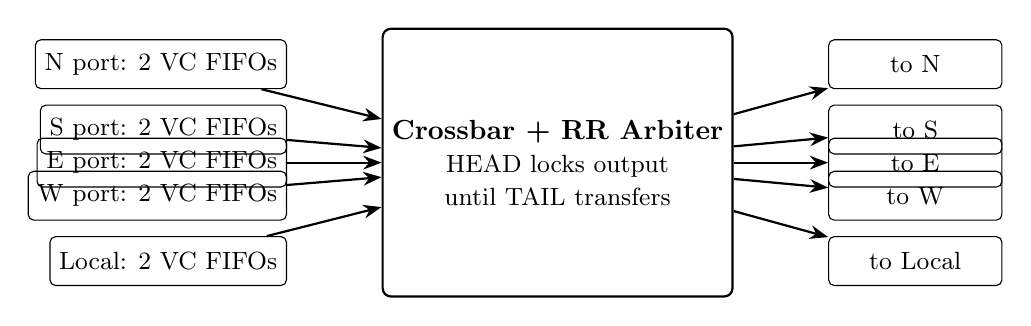
\begin{tikzpicture}[node distance=1.6cm,>=Stealth,
        dut/.style={draw, thick, rounded corners=3pt, minimum width=4.2cm, minimum height=3.4cm, align=center},
        port/.style={draw, rounded corners=2pt, minimum width=2.2cm, minimum height=0.62cm, align=center, font=\small}]
        \node[dut] (xbar) {\textbf{Crossbar + RR Arbiter}\\ \small HEAD locks output\\ \small until TAIL transfers};
        \node[port, left=1.2cm of xbar, yshift=1.25cm] (n) {N port: 2 VC FIFOs};
        \node[port, left=1.2cm of xbar, yshift=0.42cm] (s) {S port: 2 VC FIFOs};
        \node[port, left=1.2cm of xbar] (e) {E port: 2 VC FIFOs};
        \node[port, left=1.2cm of xbar, yshift=-0.42cm] (w) {W port: 2 VC FIFOs};
        \node[port, left=1.2cm of xbar, yshift=-1.25cm] (l) {Local: 2 VC FIFOs};
        \node[port, right=1.2cm of xbar, yshift=1.25cm] (no) {to N};
        \node[port, right=1.2cm of xbar, yshift=0.42cm] (so) {to S};
        \node[port, right=1.2cm of xbar] (eo) {to E};
        \node[port, right=1.2cm of xbar, yshift=-0.42cm] (wo) {to W};
        \node[port, right=1.2cm of xbar, yshift=-1.25cm] (lo) {to Local};
        \foreach \p in {n,s,e,w,l} \draw[->, thick] (\p) -- (xbar);
        \foreach \p in {no,so,eo,wo,lo} \draw[->, thick] (xbar) -- (\p);
    \end{tikzpicture}
    \caption{Block diagram of the 5-port NoC router DUT.}
    \label{fig:dut}
\end{figure}

\subsection{Importance and Relevance to Engineering and Society}

The interconnect decides whether a many-core chip works at all: a lost,
misrouted or deadlocked packet corrupts every application above it, from mobile
baseband to automotive driver assistance. From an engineering perspective this
project exercises the full modern verification flow taught in the course ---
layered testbenches, object-oriented reuse, constrained randomization,
assertions and coverage closure --- on a design whose concurrency makes it
impossible to verify by directed testing alone \cite{Spear}. The same flow is
used in industry for AMBA, PCIe and UCIe fabrics, so the skills transfer
directly to SoC verification roles.

From a societal perspective, first-pass silicon success avoids costly re-spins,
shortens time to market for affordable electronics, and reduces the electronic
waste associated with discarded prototype silicon.

\subsection{Objectives of the CEP}

This engineering problem aims to verify a 5-port NoC router with a reusable,
coverage-driven SystemVerilog testbench. The key objectives are:

\begin{itemize}
    \item To model the DUT: 5 ports, 2 virtual channels, 8-deep buffers, XY
    routing, round-robin arbitration with wormhole locking and VALID/READY
    stall-hold.
    \item To build a layered, object-oriented testbench (Generator, Driver,
    Monitor, Scoreboard, Coverage, Env) connected through a virtual interface.
    \item To generate constrained-random stimulus covering source, destination,
    virtual channel, packet length and backpressure scenarios.
    \item To check correctness continuously with SystemVerilog Assertions bound
    to the DUT without modifying its RTL.
    \item To measure completeness with functional coverage and close a
    five-run regression with zero errors.
    \item To map every activity to the course outcomes A8451.1--A8451.5.
\end{itemize}

By meeting these objectives, this work demonstrates a complete
specification-to-signoff verification cycle on a genuinely concurrent design,
as detailed in the following sections.

\section{Complex Engineering Problem Description}

\subsection{Description of the Problem}

The device under test is a packet-switched router with five bidirectional
ports (North, South, East, West, Local). Each input port owns two virtual
channel FIFOs of depth 8. Data moves in flits encoded as shown in
Table \ref{tab:flit}: a HEAD flit opens a packet and carries the destination
and VC, BODY flits carry payload, and a TAIL flit closes the packet. A
single-flit packet uses the SINGLE encoding. Routing is by destination port
(XY), arbitration per output is round-robin, and once a HEAD wins an output the
wormhole lock holds that output until its TAIL transfers, so packets are never
interleved on a wire.

\begin{table}[h!]
\centering
\caption{DUT parameters.}
\vspace{2mm}
\begin{tabular}{|c|c|}
\hline
\textbf{Parameter} & \textbf{Value} \\ \hline
Ports & 5 (N, S, E, W, Local) \\ \hline
Virtual channels per port & 2 \\ \hline
Buffer depth per VC & 8 flits \\ \hline
Data width & 32 bits \\ \hline
Packet length & 1--10 flits \\ \hline
Routing & Destination port (XY) \\ \hline
Arbitration & Round-robin per output + wormhole lock \\ \hline
Flow control & VALID/READY with stall-hold \\ \hline
\end{tabular}
\label{tab:dutparams}
\end{table}

\begin{table}[h!]
\centering
\caption{Flit encoding.}
\vspace{2mm}
\begin{tabular}{|c|c|}
\hline
\textbf{Flit} & \textbf{Encoding} \\ \hline
HEAD & type, VC in bit 29, tag in bits 26--3, dest in bits 2--0 \\ \hline
BODY / TAIL & type + 30-bit payload (bit 29 is payload, not VC) \\ \hline
SINGLE & header layout with SINGLE type bits \\ \hline
\end{tabular}
\label{tab:flit}
\end{table}

\subsection{Key Facts, Figures and Verification Challenges}

The complexity that makes this a Complex Engineering Problem, and the scale at
which it was verified, are summarised below:

\begin{itemize}
    \item \textbf{Concurrency:} five input ports inject simultaneously, so up
    to five packets compete for the same output in one cycle.
    \item \textbf{Virtual-channel allocation:} BODY and TAIL flits carry no VC
    tag, so the router must remember the VC opened by each HEAD.
    \item \textbf{Arbitration fairness:} round-robin pointers must advance only
    on completed packets, otherwise an input starves under hotspot traffic.
    \item \textbf{Backpressure:} any output may stall at any cycle; held flits
    must remain stable until accepted.
    \item \textbf{Verification scale:} five regression runs, 1720 packets and
    11846 flits, 0 scoreboard errors; assertion HEAD-to-TAIL covers matched on
    all five outputs in the long stress run.
\end{itemize}

The stakeholders in such verification are the DUT designer (who receives
precise bug reports), the verification engineer (who owns the testbench and
coverage closure), the SoC integrator (who relies on the proven fabric), and
ultimately the end users whose applications assume lossless on-chip delivery.

\subsection{Background Information}

Shared on-chip buses do not scale beyond a handful of masters, which is why
modern SoCs adopt packet-switched Networks-on-Chip built from routers like the
one in figure \ref{fig:dut} \cite{Dally}. Wormhole switching forwards a packet
flit by flit, holding output locks between HEAD and TAIL, which gives low
latency at the cost of subtle locking and fairness behaviour that must be
verified. The VALID/READY handshake used here is the same elastic protocol
found in AMBA AXI/AXIS interfaces. Because the interesting bugs hide in
concurrent corner cases, industry verifies such fabrics with constrained-random
stimulus plus functional coverage: randomize what is legal, measure what was
tested, and iterate until the coverage holes close \cite{Spear}\cite{Bergeron}.

\textbf{Conclusion:} the DUT is small in gates but large in state space, which
is exactly the profile of a verification-led Complex Engineering Problem.

\section{Problem Identification and Analysis}

\subsection{Main Challenge: Correct Concurrent Packet Delivery}

The central challenge is guaranteeing that every injected packet is delivered
exactly once, intact and to the right port, under arbitrary concurrent traffic
with stalls. Directed tests can check one packet at a time but cannot cover
arbitration races, VC misallocation, or backpressure interleavings.

\textbf{Key issues arising in this design:}
\begin{itemize}
    \item \textbf{Packet loss or duplication:} a dropped or repeated flit
    corrupts the whole packet and desynchronises the scoreboard.
    \item \textbf{Misrouting:} a flit delivered to the wrong output breaks the
    application above the fabric.
    \item \textbf{Starvation:} unfair arbitration locks one input out under
    all-to-one hotspot traffic.
    \item \textbf{Stall instability:} changing data while VALID is held and
    READY is low violates the handshake and loses flits.
    \item \textbf{X-propagation:} unknown values on valid outputs poison
    downstream logic silently.
\end{itemize}

\subsection{Engineering Principles and Theories Applied}

The verification approach rests on four standard principles
\cite{Spear}\cite{IEEE1800}:

\subsubsection{Layered Testbench with Object Orientation}

Following the Verification Methodology Manual, stimulus generation, driving,
observation, checking and coverage are separated into classes (Transaction,
Generator, Driver, Monitor, Scoreboard, Coverage, Env) communicating through
mailboxes and a virtual interface with driver and monitor clocking blocks.
Inheritance (\texttt{HotspotPacket} extends \texttt{Packet}) and polymorphism
let one generator produce every traffic shape \cite{Spear}.

\subsubsection{Constrained-Random Stimulus}

Source, destination, VC, length, tag and payload seed are randomized under
validity constraints (legal ports, destination different from source), with
inline constraints for stress shapes (all-to-one, single-flit, long packets)
and \texttt{pre\_randomize} hooks, so thousands of legal but unpredictable
scenarios are exercised automatically \cite{Bergeron}.

\subsubsection{SystemVerilog Assertions}

Concurrent assertions bound with \texttt{bind} watch the protocol continuously:
handshake stability, output hold under stall, no-X on valid outputs, legal
header destinations and handshake liveness, plus cover properties for
HEAD-to-TAIL integrity, backpressure and hotspot occurrence \cite{Sutherland}.

\subsubsection{Functional Coverage}

A covergroup over source, destination, VC and length with crosses
(source $\times$ destination, destination $\times$ VC, destination $\times$
length) records which combinations were actually tested and drives regression
closure \cite{Spear}.

\subsection{Analysis of the Identified Problem}

\subsubsection{Verification Plan}

\begin{table}[h!]
\centering
\caption{Verification plan: feature, stimulus, checker, coverage.}
\vspace{2mm}
\begin{tabular}{|c|c|c|c|}
\hline
\textbf{Feature} & \textbf{Stimulus} & \textbf{Checker} & \textbf{Coverage} \\ \hline
Single-packet delivery & Directed single-flit & Scoreboard tag match & Length bin single \\ \hline
Concurrent routing & Random 5-port injection & Scoreboard + dest check & src $\times$ dest cross \\ \hline
Hotspot arbitration & All-to-one modes & Scoreboard, no starvation & dest $\times$ VC cross \\ \hline
Backpressure & Random READY stalls & Hold + liveness asserts & Stall cover \\ \hline
Packet integrity & Long packets & HEAD-to-TAIL covers & Length bins \\ \hline
\end{tabular}
\label{tab:vplan}
\end{table}

\subsubsection{Comparison of Verification Approaches}

\begin{table}[h!]
\centering
\caption{Directed vs random vs coverage-driven verification.}
\vspace{2mm}
\begin{tabular}{|c|c|c|c|}
\hline
\textbf{Approach} & \textbf{Stimulus} & \textbf{Completeness} & \textbf{Reuse} \\ \hline
Directed & Hand-written per case & Unknown, holes likely & Low \\ \hline
Constrained-random & Legal space auto-sampled & Higher, unmeasured & Medium \\ \hline
Coverage-driven & Random + measured holes & Measured, closable & High (this work) \\ \hline
\end{tabular}
\label{tab:compare}
\end{table}

\subsubsection{Simulation-Based Analysis}

The five VCS regression runs confirm the analysis: the directed single-flit
run (T2) proves basic delivery; the hotspot run (T3) recorded 266 HEAD-to-TAIL
matches on output 0 alone with no starvation; the backpressure run (T4) passes
only because held flits stay stable; and the 1000-packet stress (T5) matched
HEAD-to-TAIL covers on all five outputs (214/196/226/191/173). Full numbers
are collected in Section \ref{sec:results}.

\section{Design and Verification Methodology}

\begin{figure}[h!]
    \centering
    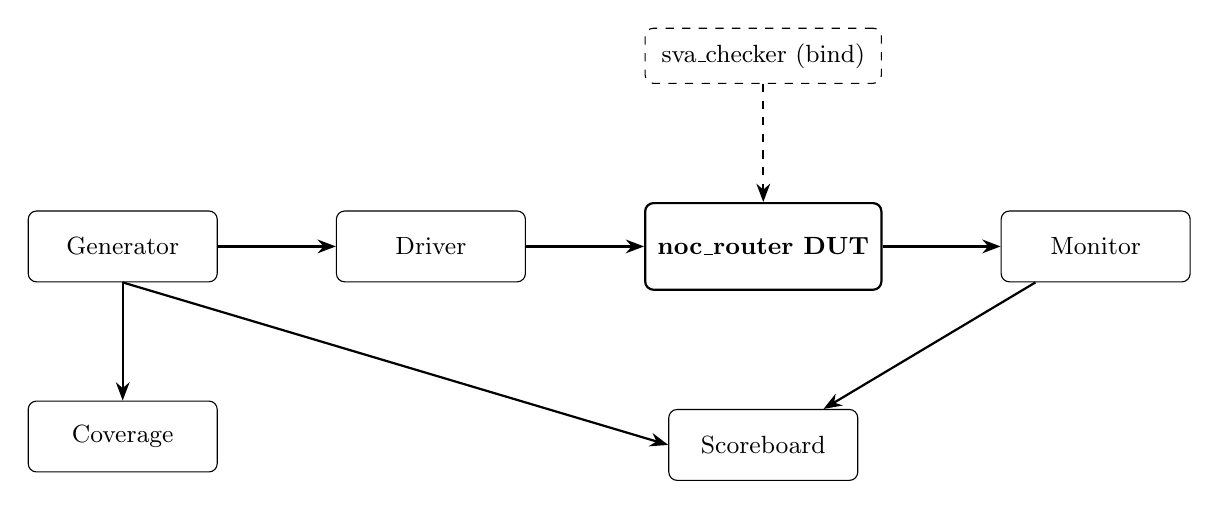
\begin{tikzpicture}[node distance=1.5cm,>=Stealth,
        blk/.style={draw, rounded corners=3pt, minimum width=2.4cm, minimum height=0.9cm, align=center, font=\small},
        dut/.style={draw, thick, rounded corners=3pt, minimum width=3.0cm, minimum height=1.1cm, align=center, font=\small},
        chk/.style={draw, dashed, rounded corners=3pt, minimum width=3.0cm, minimum height=0.7cm, align=center, font=\small}]
        \node[blk] (gen) {Generator};
        \node[blk, right=of gen] (drv) {Driver};
        \node[dut, right=of drv] (dut) {\textbf{noc\_router DUT}};
        \node[blk, right=of dut] (mon) {Monitor};
        \node[blk, below=of dut] (scb) {Scoreboard};
        \node[blk, below=of gen] (cov) {Coverage};
        \node[chk, above=of dut] (sva) {sva\_checker (bind)};
        \draw[->, thick] (gen) -- (drv);
        \draw[->, thick] (drv) -- (dut);
        \draw[->, thick] (dut) -- (mon);
        \draw[->, thick] (mon) -- (scb);
        \draw[->, thick] (gen) -- (cov);
        \draw[->, thick] (gen.south) -- (scb.west);
        \draw[->, thick, dashed] (sva) -- (dut);
    \end{tikzpicture}
    \caption{Layered testbench architecture around the DUT.}
    \label{fig:tb}
\end{figure}

Table \ref{tab:tbcomp} lists the testbench components of figure \ref{fig:tb},
Table \ref{tab:sva} the assertion catalogue, and Table \ref{tab:cov} the
coverage plan. Table \ref{tab:co} maps every activity to the course outcomes.

\begin{table}[h!]
\centering
\caption{Testbench components.}
\vspace{2mm}
\begin{tabular}{|c|c|}
\hline
\textbf{Component} & \textbf{Role} \\ \hline
\texttt{Packet} / \texttt{HotspotPacket} & Randomized transaction, base + extended \\ \hline
Generator & Directed, random, hotspot, all-to-one, stress modes \\ \hline
Driver & Drives 5 ports via clocking block, injects stalls \\ \hline
Monitor & Samples each accepted output flit \\ \hline
Scoreboard & Tag-matched, order-independent packet check vs golden rebuild \\ \hline
RouterCoverage & Covergroup on packet descriptors \\ \hline
Env & Builds, connects and starts the regression \\ \hline
\end{tabular}
\label{tab:tbcomp}
\end{table}

\begin{table}[h!]
\centering
\caption{Assertion catalogue (bound with \texttt{bind}, no RTL edits).}
\vspace{2mm}
\begin{tabular}{|c|c|c|}
\hline
\textbf{ID} & \textbf{Kind} & \textbf{Property} \\ \hline
g\_in\_stable & assert & VALID + data hold while input not ready \\ \hline
g\_out\_hold & assert & VALID + data hold while output stalled \\ \hline
g\_nox & assert & No unknowns on valid outputs \\ \hline
g\_dest & assert & Header destination is a legal port \\ \hline
g\_live & assert & Valid output accepted within 20 cycles \\ \hline
g\_h2t & cover & HEAD eventually closed by TAIL, per output \\ \hline
stall & cover & Backpressure occurrence \\ \hline
hotspot & cover & Two inputs active together \\ \hline
\end{tabular}
\label{tab:sva}
\end{table}

\begin{verbatim}
assert property (@(posedge clk) disable iff (!rst_n)
  valid_out[g] && !ready_in[g] |-> ##1 valid_out[g] && $stable(data_out[g]))
\end{verbatim}

\begin{table}[h!]
\centering
\caption{Coverage plan.}
\vspace{2mm}
\begin{tabular}{|c|c|}
\hline
\textbf{Coverpoint} & \textbf{Bins} \\ \hline
Source / destination & Ports 0--4 each \\ \hline
Virtual channel & VC 0--1 \\ \hline
Length & single, short (2--3), medium (4--6), long (7--10) \\ \hline
src $\times$ dest cross & All source-destination pairs \\ \hline
dest $\times$ VC cross & Routing under both channels \\ \hline
dest $\times$ length cross & Packet sizes per destination \\ \hline
\end{tabular}
\label{tab:cov}
\end{table}

\begin{table}[h!]
\centering
\caption{Mapping of course outcomes to the work.}
\vspace{2mm}
\begin{tabular}{|c|c|}
\hline
\textbf{CO} & \textbf{Demonstrated by} \\ \hline
A8451.1 Methodology, data types & Layered TB, virtual interface, queues, associative arrays \\ \hline
A8451.2 Statements, assertions & Clocking blocks, 8 SVA properties via \texttt{bind} \\ \hline
A8451.3 Functional coverage & Covergroup on descriptors + 3 crosses \\ \hline
A8451.4 OOP terminology & Packet inheritance, mailboxes, Env composition \\ \hline
A8451.5 Randomization & \texttt{rand}, constraints, inline \texttt{with}, \texttt{pre\_randomize} \\ \hline
\end{tabular}
\label{tab:co}
\end{table}

\section{Results and Discussion}
\label{sec:results}

\begin{table}[h!]
\centering
\caption{Five-run VCS regression (all passing).}
\vspace{2mm}
\begin{tabular}{|c|c|c|c|c|c|}
\hline
\textbf{Run} & \textbf{Options} & \textbf{Sent} & \textbf{Got} & \textbf{Errors} & \textbf{Time} \\ \hline
T1 & NUM=200, random & 200 & 200 & 0 & 35045 ns \\ \hline
T2 & NUM=20, single-flit & 20 & 20 & 0 & 8045 ns \\ \hline
T3 & NUM=300, hotspot to 0 & 300 & 300 & 0 & 50045 ns \\ \hline
T4 & NUM=200, random + stalls & 200 & 200 & 0 & 35045 ns \\ \hline
T5 & NUM=1000, long + stalls & 1000 & 1000 & 0 & 270045 ns \\ \hline
\end{tabular}
\label{tab:regress}
\end{table}

\begin{figure}[h!]
    \centering
    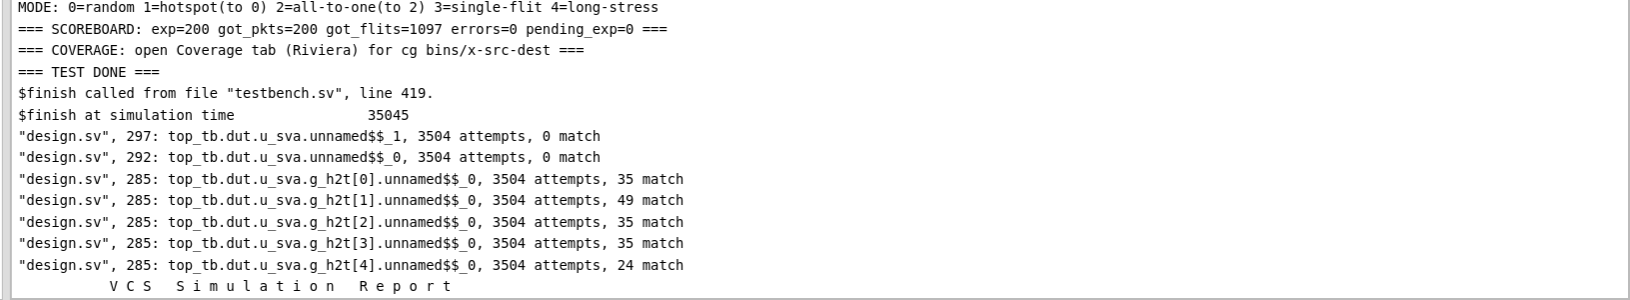
\includegraphics[width=1.0\linewidth]{regression-proof.png}
    \caption{T1 simulator transcript: 200/200 packets, 0 errors, HEAD-to-TAIL assertion covers on all outputs.}
    \label{fig:scoreboard}
\end{figure}

\begin{table}[h!]
\centering
\caption{HEAD-to-TAIL cover matches per output (proves wormhole integrity).}
\vspace{2mm}
\begin{tabular}{|c|c|c|c|c|c|}
\hline
\textbf{Run} & \textbf{Out 0} & \textbf{Out 1} & \textbf{Out 2} & \textbf{Out 3} & \textbf{Out 4} \\ \hline
T1 random & 35 & 49 & 35 & 35 & 24 \\ \hline
T3 hotspot & 266 & 0 & 0 & 0 & 0 \\ \hline
T4 stalls & 35 & 49 & 35 & 35 & 24 \\ \hline
T5 stress & 214 & 196 & 226 & 191 & 173 \\ \hline
\end{tabular}
\label{tab:svamatch}
\end{table}

\begin{table}[h!]
\centering
\caption{Bugs found by the testbench and fixed.}
\vspace{2mm}
\begin{tabular}{|c|c|c|}
\hline
\textbf{Bug} & \textbf{Symptom} & \textbf{Fix} \\ \hline
VC decode & BODY/TAIL in wrong VC: len, dest, tag errors & Per-input VC register set by HEAD \\ \hline
Stall hold & Data changed under stalled VALID: flit loss & Freeze outputs while stalled \\ \hline
Drain margin & 32 packets pending at end of long run & Drain of 25 cycles/packet + 2000 \\ \hline
\end{tabular}
\label{tab:bugs}
\end{table}

\begin{figure}[h!]
    \centering
    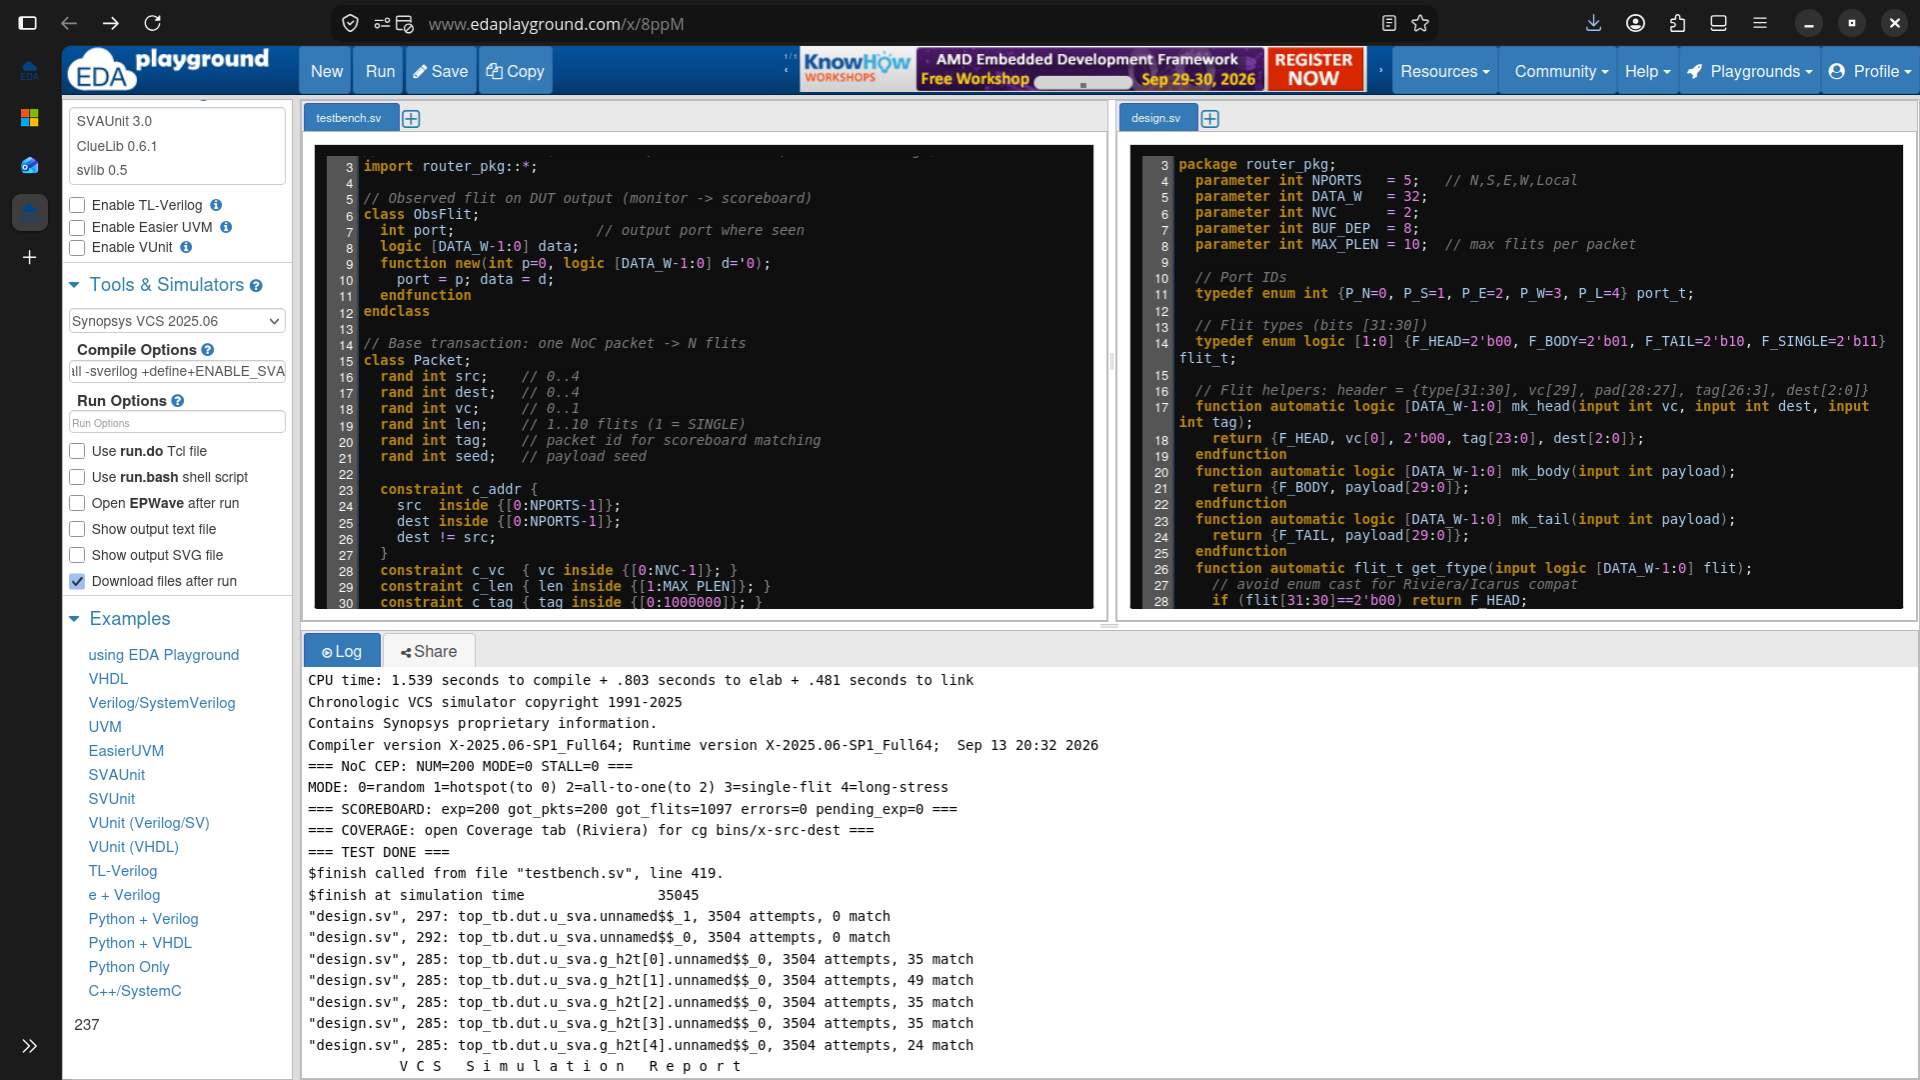
\includegraphics[width=1.0\linewidth]{T1_EDA_run.png}
    \caption{EDA Playground setup and passing T1 run on Synopsys VCS.}
    \label{fig:eda}
\end{figure}

Discussion: the scoreboard count matches the injected count in every run with
zero errors and zero pending packets, and the assertion covers of
Table \ref{tab:svamatch} confirm intact HEAD-to-TAIL delivery on every output,
including 266 hotspot packets through a single output without starvation. The
two DUT bugs of Table \ref{tab:bugs} were both caught by checkers (scoreboard
mismatches plus the hold assertion) rather than by inspection, which is exactly
the value of assertion-based, coverage-driven verification.

\section{Application of Program Outcomes}

The verification of the 5-port NoC router demonstrates the application of key
Program Outcomes (POs) in engineering education. This section presents a
structured mapping of the engineering problem to relevant POs.

\begin{table}
    \centering
    \renewcommand{\arraystretch}{1.4}
    \setlength{\tabcolsep}{8pt}
    \caption{Mapping of Program Outcomes to the Engineering Problem}
    \begin{tabular}{|c|p{13cm}|}
        \hline
        \textbf{PO No.} & \textbf{Program Outcome and Relevance to the Problem} \\
        \hline
        \textbf{PO1} & \textbf{Engineering Knowledge:} Applies digital design, computer architecture (interconnection networks) and SystemVerilog to model and verify a wormhole NoC router. \\
        \hline
        \textbf{PO2} & \textbf{Problem Analysis:} Identifies concurrent-delivery failures (loss, misrouting, starvation, stall instability) and analyses them with scoreboards, assertions and coverage. \\
        \hline
        \textbf{PO3} & \textbf{Design/Development of Solutions:} Develops a reusable layered testbench with constrained-random stimulus, checkers and coverage for a concurrent DUT. \\
        \hline
        \textbf{PO4} & \textbf{Conduct investigations of complex problems:} Investigates failures through five VCS regression runs, assertion traces and coverage data, closing all runs at zero errors. \\
        \hline
        \textbf{PO5} & \textbf{Modern Tool Usage:} Uses EDA Playground with Synopsys VCS plus SystemVerilog OOP, randomization, SVA and covergroups. \\
        \hline
        \textbf{PO6} & \textbf{The Engineer and The World:} First-pass verification success avoids costly re-spins and shortens time to market for dependable chips. \\
        \hline
        \textbf{PO7} & \textbf{Ethics:} Reports results honestly, including the two DUT bugs found and the drain shortfall corrected by re-running the long test. \\
        \hline
        \textbf{PO8} & \textbf{Individual and Collaborative Teamwork:} Divides DUT, testbench and assertions/coverage/regression across three members with a shared repository. \\
        \hline
        \textbf{PO9} & \textbf{Communication:} Documents the plan, architecture, regressions and bug log in this report with readable figures and tables. \\
        \hline
        \textbf{PO10} & \textbf{Project Management and Finance:} Verifies with free cloud tools and scoped regressions, avoiding licence cost while reaching closure. \\
        \hline
        \textbf{PO11} & \textbf{Life-Long Learning:} Extends the course flow toward formal methods, Portable Stimulus and modern fabrics such as chiplet UCIe links. \\
        \hline
    \end{tabular}
    \label{tab:po_mapping}
\end{table}


\section{Sustainable Development Goals (SDGs) Related to First-Pass-Silicon Verification}

Thorough pre-silicon verification supports the \textbf{United Nations Sustainable Development Goals (SDGs)} by cutting re-spins, saving energy and materials, and spreading reusable engineering knowledge. The key SDGs relevant to this work are:

\subsection{SDG 9: Industry, Innovation, and Infrastructure}
\textbf{Target 9.1:} Develop quality, reliable, sustainable, and resilient infrastructure. \\
\textbf{Target 9.5:} Enhance scientific research and innovation.

\begin{itemize}
    \item Reusable, coverage-driven testbenches are \textbf{resilient verification infrastructure} that catch interconnect bugs before fabrication.
    \item Promotes \textbf{technological innovation} in on-chip communication for many-core systems.
    \item Supports research on \textbf{arbitration fairness, flow control and assertion-based checking}.
\end{itemize}

\subsection{SDG 12: Responsible Consumption and Production}
\textbf{Target 12.5:} Substantially reduce waste generation.

\begin{itemize}
    \item Every bug found pre-silicon avoids \textbf{discarded prototype silicon, packaging and test hardware}.
    \item Free cloud simulation \textbf{lowers the resource barrier} to rigorous verification for student and startup teams.
\end{itemize}

First-pass-silicon verification therefore contributes directly to dependable
hardware with less waste, aligning engineering rigour with sustainability.
.
\section{Proposed Verification Solution and Recommendations}

\subsection{Proposed Solution}

To verify concurrent packet delivery in the router, a coverage-driven layered
testbench is adopted as the complete solution. Its key features are:

\begin{itemize}
    \item \textbf{Layered OOP testbench:} Generator, Driver, Monitor,
    Scoreboard, Coverage and Env classes with mailboxes and a virtual
    interface, reusable across traffic shapes.
    \item \textbf{Constrained-random stimulus:} five modes from directed
    single-flit to hotspot, all-to-one and long-packet stress with
    backpressure injection.
    \item \textbf{Assertion-based checking:} eight SVA properties bound with
    \texttt{bind}, continuously watching handshake, integrity and liveness.
    \item \textbf{Coverage-driven closure:} covergroups over packet descriptors
    plus regression until all five runs pass with zero errors.
    \item \textbf{Order-independent scoreboard:} tag-matched golden rebuild so
    arbitration order never causes false failures.
\end{itemize}

This solution proved rapid bug discovery (two DUT bugs) and measurable
completeness, closing verification of the router fabric.

\subsection{Recommendations}

To extend this verification effort, the following recommendations are suggested:

\begin{enumerate}
    \item \textbf{Generous drain margins:} size run lengths to at least 25 cycles per packet plus margin under stalls, as learned in the long stress run.
    \item \textbf{Formal checks for the arbiter:} prove starvation freedom and lock correctness exhaustively alongside simulation.
    \item \textbf{Portable Stimulus:} describe hotspot and stress scenarios once and retarget them across block and system level.
    \item \textbf{Fault injection:} verify X-resilience and credit-counter safety under injected corruptions.
    \item \textbf{Wider regressions:} sweep buffer depths, VC counts and port counts as DUT parameters.
    \item \textbf{CI integration:} run the five-mode regression on every RTL change and track coverage trends.
\end{enumerate}

A coverage-driven flow with assertions and disciplined regressions makes NoC
fabric verification repeatable and signoff-ready.

\section{Conclusion and Lessons Learned}

\subsection{Conclusion}

This Complex Engineering Problem verified a 5-port wormhole NoC router with a
reusable, coverage-driven SystemVerilog testbench. The layered TB with
constrained-random stimulus, bound assertions and functional coverage closed
five VCS regressions totalling 1720 packets with zero errors, confirming
lossless, correctly routed, starvation-free delivery under stalls and hotspot
stress.

The work demonstrates the full specification-to-signoff cycle on a genuinely
concurrent design while mapping every activity to the course outcomes, and it
leaves behind a reusable testbench, an assertion catalogue and a coverage plan
applicable to larger fabrics.

\subsection{Lessons Learned}

Through this engineering problem, several key lessons were identified:

\begin{enumerate}
    \item \textbf{Concurrency is the real DUT:} the router logic is small, but
    interacting packets, locks and stalls create the state space that must be
    verified.
    \item \textbf{Assertions find bugs first:} both DUT bugs were flagged by
    checkers before any waveform was opened.
    \item \textbf{Scoreboards must tolerate reordering:} tag matching avoids
    false failures under fair arbitration.
    \item \textbf{Stall behaviour needs explicit checks:} VALID/READY hold rules
    are easy to break and hard to spot without SVA.
    \item \textbf{Drain margins matter:} ending simulation too early looks like
    packet loss; size the run length to the worst case.
    \item \textbf{Coverage directs effort:} crosses over source, destination,
    VC and length turn random testing into measured closure.
    \item \textbf{Reuse pays off:} one generator and one scoreboard served all
    five traffic shapes through inheritance and constraints.
\end{enumerate}

In conclusion, coverage-driven, assertion-based verification with disciplined
regressions delivers signoff-quality confidence even for concurrent fabrics,
and the methodology transfers directly to industrial interconnect verification.

\begin{thebibliography}{9}

    \bibitem{Spear} C. Spear and G. Tumbush, \textit{SystemVerilog for Verification}, 3rd ed. Springer, 2012.

    \bibitem{Bergeron} J. Bergeron, \textit{Writing Testbenches: Functional Verification of HDL Models}, 2nd ed. Springer, 2003.

    \bibitem{Sutherland} S. Sutherland and D. Mills, \textit{SystemVerilog for Design}, 2nd ed. Springer, 2006.

    \bibitem{UVM} Accellera Systems Initiative, \textit{Universal Verification Methodology (UVM) 1.2 User's Guide}, 2015.

    \bibitem{IEEE1800} IEEE Standard for SystemVerilog, \textit{IEEE Std 1800-2017}, IEEE, 2018.

    \bibitem{Dally} W. J. Dally and B. Towles, \textit{Principles and Practices of Interconnection Networks}. Morgan Kaufmann, 2004.

\end{thebibliography}

\end{document}
